What an application (or ``app'') \emph{does} is not always what a user
\emph{expects}.
User expectations stem from user perceptions (information they can perceive about an app).
As shown in Figure~\ref{fig:Problem}, user perceptions come from two main sources:
app descriptions form user perception before installation, and user interfaces
enrich user perception after installation.
Two types of inconsistencies, corresponding to each of these sources, contribute
to the gap between app behavior and user perception.
(1) Install-time inconsistency involves the functionalities described in app
descriptions being inconsistent with the actual app behaviors.
% An app developer may produce fake or incomplete app descriptions to trick users
% into installing the app.
(2) Run-time inconsistency involves the behavior indicated through user
interfaces (external behavior) being inconsistent with the behavior running in
the background (internal behavior).
% An app developer may camouflage malicious behavior in the background while
% showing users the benign behaviors on the interfaces.
In this proposal, we aim to bridge the gap between user perception and app
behavior by developing a set of automated analyses to check these two
inconsistencies and warn users about potential risks.

As an example of how install-time inconsistency is manifested, consider
installing an app on a system with permissions that guard access to
sensitive resources.
% The privileges for an application (i.e.\ app) to access sensitive resources are
% granted through a permission system on modern desktop and mobile operating
% systems.
% An ideal permission system should inform users of potential risks and empower
% users in making security decisions~\cite{felt2012ask}.
The permission system from earlier versions of Android up to Android Marshmallow
ask users to grant access to a list of permissions when an app is installed.
Unfortunately, a list of permissions and an app description are
insufficient for users to understand the potential risks in apps.
A recent study~\cite{felt2012android} suggests that users find the Android
permission system hard to understand because ``there is no way to know what app
functionality the install-time permissions correspond to.''
Another study~\cite{chin2012measuring} reveals that if users are aware of when
the permission will be used in the app, they will trust the app more. For
example, a majority of participants feel more comfortable using location
services on navigation apps because they can perceive the use of that permission.

In more recent versions of Android (Android Marshmallow or higher), the system can ask
its users to grant each permission as the permission is needed by the app.
This new permission system exists so that users can decide to grant access to the
requested permissions with better context as to what the app might be
using them for.
However, one can imagine that even with this new permission system of Android,
developers with malicious intent can still deceive users to grant them access
to permissions that the app may exploit.
For example, an app that sends SMS messages 
could also upload the contacts' information to a remote
malicious server. Although the context for obtaining the
contact information is legitimate, the use of the contact information is unexpected.
To better inform users of potential risks, we propose an undeceivable system that provides
contextual information generated from \emph{how} and \emph{when} permissions are used
by an app.

% Even if install-time inconsistency is alleviated by providing contextual
% information, run-time inconsistencies can still cause a gap in user perception
% and app behavior.
% For example, in the current Android permission system, users cannot ensure
% that an app only uses permissions for its claimed functionality.
% In the case of the \emph{DroidDreamLight}~\cite{balanza2011ddl} trojan, an
% information harvesting service is grafted onto existing Android apps and uploads
% user information when the phone receives any phone call. To users of infected
% applications, there may be no visible information that would indicate this
% malicious behavior, especially if the host app already requests the required
% permissions. The service would have access to all the information the host app
% can access, but uses this information in unexpected ways.

%Last, in addition to lacking the context information, the coarse granularity of permission also pose difficulty for users to decide potential risk. A single permission in Android often contains several low level capabilities that the app can gain from the permission. For example, by granting the permission "READ\_PHONE\_STATE", the app will have the capabilities to read Device Id, VoiceMail Number, Sim Serial Number, Device Software Version etc. Users, on the other hand, may expect the app only have the capability to read part of these information. In this way, the permission system cannot fully inform the users of the potential risks. Previous user study~\cite{felt2012android} also conforms to the fact. It shows that user can identify (part of) the permission definition, but they are confused about the scope of permission. Users incorrectly believe that a given permission has more capabilities or less capabilities than it actually has. So in addition to the name of permission, the information of which capability has been leveraged in the app is also important for user to make security decision.

 \begin{figure}[H]%
 \centering
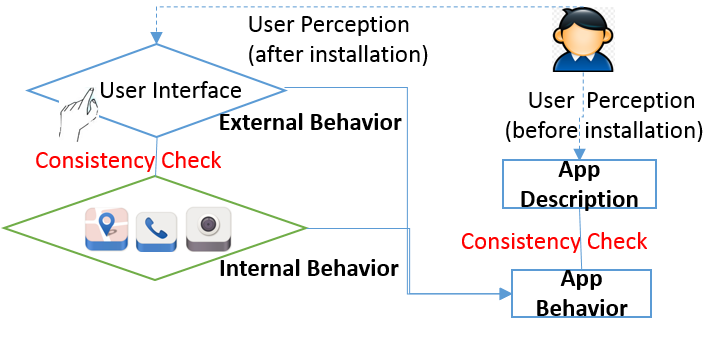
\includegraphics[width=0.38\textwidth]{Problem.png}%
\caption{User perception and app behaviors
 }%
\label{fig:Problem}%
\end{figure}

% In this proposal, we aim to validate app behaviors against user expectations of the behavior to bridge the gap between the user expectations and app behaviors. 
% The users expectations of app behaviors are indicated by the user perceptions (i.e., what users perceive from the app ).
% As shown in Figure~\ref{fig:Problem}, user perceptions come from two sources: app descriptions form user perception at installation time, and user interfaces enrich user perception after installation.
% Two potential inconsistencies may lead to the gap between user perception and app behaviors. First, the behavior indicated through user interfaces (External Behavior) can be inconsistent with the behavior running in the background (Internal Behavior).
% The app developer may camouflage malicious behavior in the background while showing users the benign behaviors on the interfaces.
% Second, the functionalities described in app descriptions can be inconsistent with the actual app behaviors. The app developer may produce fake or incomplete app descriptions to trick users into installing the app.
% In this work, we develop a set of automated analyses to check these two inconsistencies and warn users about potential risks.

% In checking install-time inconsistency, the challenge is to associate the functional behaviors in app descriptions to the non-functional behaviors (e.g., security behavior) extracted from the apps. 
Checking install-time and run-time inconsistency faces challenges.
Existing research exists for checking either inconsistency,
but none of the existing work has linked the security behaviors of an app to its
functional descriptions.
Although some existing approaches~\cite{felt2011survey,zhou2012hey,peng2012using,hornyack2011these,enck2010taintdroid,grace2012riskranker,zhou2012dissecting} analyze the security attributes (e.g., the information flows from a method reading sensitive data to methods sending the data out) of an app for security analysts to review, they do not associate the app's functionalities with these security attributes.
Therefore, security analysts are unable to make accurate decisions because the security attributes (e.g., information flows) in legitimate apps and illegitimate apps could be the same.
On the other hand, existing approaches~\cite{harman2012app, whyper} that use data mining or natural language processing techniques to analyze an app's descriptions to identify sentences that may describe the security requirements of such apps do not consider the behavior of the app. Therefore, malware developers could easily provide fake text artifacts to fool the analysis techniques in these approaches.

% Additional challenges in checking run-time inconsistency includes comparing the detailed program analysis information representing internal behaviors with natural language information (e.g., UI texts) representing external behaviors.
% Although existing approaches~\cite{robillard1986schematic, sridhara2011generating} in program comprehension can infer natural language documentation from the source code of apps, the source code of apps on the market are usually not available.
% Moreover, the result of existing approaches heavily relies on the text in the program code. Developers of the malicious app could alter the names of the program variables or methods to camouflage the app as a benign one.

%The task of providing a informative permission system is non-trivial. In addition to recover all the information needed, the representation of the information is also challenging. The challenges are two-fold; First, the representation of the information provided should be easy to understand. Average Android users should be able to understand the information without any sophisticated knowledge. Second, the information provided should be accurate and succinct. To avoid the information overload, the permission system should filter out the redundant information. The information of the permission system should not overlap with any existing information that users already know during the installation time.
%That means, any information users can infer from app description, screen shot and permission system should not be repetitive.

 \begin{figure}[H]%
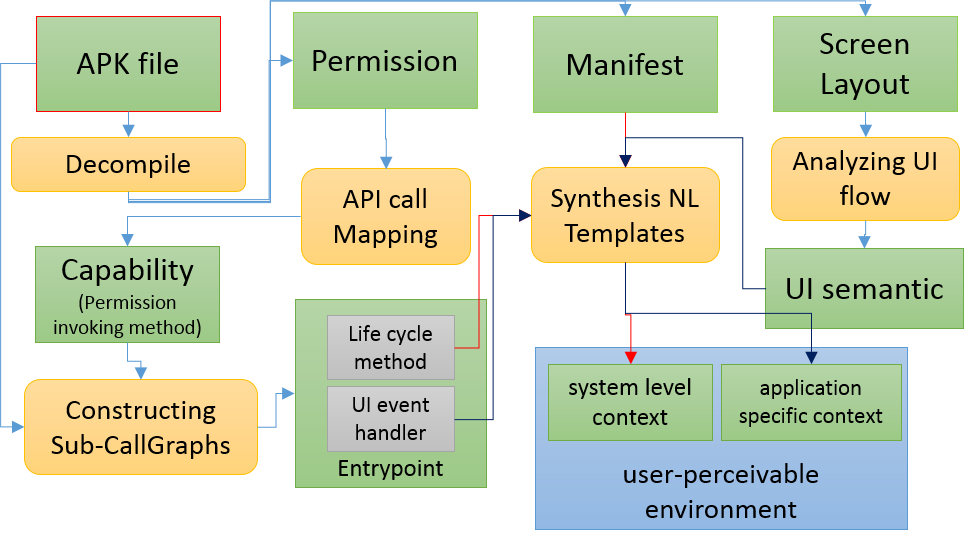
\includegraphics[width=0.46\textwidth]{User_Perceived.png}%
\caption{Overview of context recovery for permission usage
 }%
\label{fig:User_Perceived}%
\end{figure}

% To address these challenges, we propose a two-fold representation in natural language showing both the usage context for finer grained capabilities in each permission and the underlying permission usage that is inconsistent with perceived external behavior.
To address these challenges, we summarize our context recovery system for permission usage in the following three steps.
Figure~\ref{fig:User_Perceived} depicts the overview of our context recovery system for permission usage.
(1) We extract usage context by recovering the \emph{user-perceivable environment} when each permission is used. We categorize the user-perceivable environment into two categories, the \emph{system level} and the \emph{application specific} context. The system level context refers to common system events such as incoming messages and phone calls, when the device starts, etc. The application specific context represents semantics of GUI actions. To recover the context information, we construct the call graph and build a mapping between the user-perceivable context and the method that directly uses a permission. Then we develop template-based natural language synthesis techniques to generate natural language descriptions of how a permission is used under what context.
(2) We detect whether the underlying permission usage has additional behaviors, by performing taint analysis from each source (method that uses a permission) to identify its sinks (places where the sensitive data leave the app). For each sink method, we repeat the same procedure in our first step to synthesize natural language descriptions on permission usage context.
(3) We compare the synthesized descriptions with the app descriptions using documentation-similarity analysis techniques~\cite{sensim, docsim}. Since we aim to minimize the information overhead presented to users, we report back to users only when an inconsistency is found.

% First, to extract usage context, we recover the \emph{user-perceivable environment} when each permission is used. We categorize the user-perceivable environment into two categories, the \emph{system level} and the \emph{application specific} context. The system level context refers to common system events such as incoming messages and phone calls, when the device starts, etc. The application specific context represents semantics of GUI actions. To recover the context information, we construct the call graph and build a mapping between the user-perceivable context and the method that directly uses a permission. Then we use template-based natural language synthesis techniques to generate natural language descriptions of how a permission is used under what context.

% Second, to detect whether the underlying permission usage has additional behaviors, we perform a taint analysis from each source (method that uses a permission) to identify its sinks (places where the sensitive data leave the app). For each sink method, we repeat the same procedure in our first step to synthesize natural language descriptions on permission usage context.

% Last, we compare the synthesized descriptions with the app descriptions using existing documentation similarity-analysis techniques~\cite{sensim, docsim}. Since we aim to minimize the information overhead presented to users, we only report back to users when an inconsistency is found.

%To map the usage of capabilities to the phone system events and GUI events, we construct the call graphs containing permission related methods. The entry points of the call graphs are either GUI event handlers or Android component life cycle methods. We then analyze the app manifest to obtain the system event information that can invoke life cycle methods.  To synthesize description of permission usage based on the context information, we employ pre-defined natural-language templates for explaining permission usage~\cite{Sai01doc4test}, and automatically fill in the contents of the templates as the descriptions. In particular, we will define templates for describing common usage contexts, such as making phone calls, sending emails, and searching for nearby shops, and fill the contents based on the contexts information produced by the previous step.

%Second, to detect and represent the underlying permission usage inconsistent with claimed functionality,  we will also define templates for describing how the permission will be used. We will first locate the SDK methods send out private information based on the computation of information flows and then we use the description of these methods in API documents to synthesized sentences describing underlying permission usage. We will also synthesize user-perceivable context information for these SDk methods by applying the techniques in the first part of our approach. We compare the synthesized sentences of underlying permission usage to the related sentences in app descriptions as well as synthesized sentences of the user-perceivable context. The challenge is how to compute the similarities between these sentences to identify inconsistencies. We plan to adapt the existing documentation/sentence similarity-based techniques~\cite{sensim, docsim} by assigning more weights to permission-related keywords based on our knowledge graph~\cite{whyper}, and incorporate semantic information that we can obtain from the natural-language processing techniques employed in our existing work whyper~\cite{whyper}, such as dependency information and part-of-speech tags.

% As , the current Android permission system is n ;
%  The information provided by permission system is not enough for
%of whether to install an application or notTo provide a informative is non-trivial.